\documentclass[a4paper,12pt]{article}
\usepackage[utf8]{inputenc}
\usepackage[T1]{fontenc}
\usepackage[french]{babel}
\usepackage{graphicx}
\usepackage{hyperref}
\usepackage{geometry}
\usepackage{xcolor}
\usepackage{tikz}
\usetikzlibrary{calc}
\geometry{margin=2.5cm}


\usepackage{float}
\begin{document}


\begin{tikzpicture}[remember picture,overlay]
    % Bordure
    \node[anchor=north west] at (current page.north west) 
        {\includegraphics[width=2cm,height=14cm,keepaspectratio]{Bordure.png}};
    
    \node[anchor=north west] (logo_text) at ($(current page.north west)+(2cm,-0.2cm)$) {
        \includegraphics[width=2.3cm]{logo_nanterre.png}%
        \hspace{0.3cm}%
        \begin{minipage}[b]{10cm}  
            \large \textbf{UNIVERSITÉ PARIS NANTERRE} \\
            \vspace{0.3cm}  
        \end{minipage}
    };
\end{tikzpicture}

\vspace*{2cm} 

\begin{center}
    \Large Licence MIASHS deuxième année
\end{center}

\vspace*{1cm}
\begin{center}
    \huge \textbf{Rapport de projet informatique}
\end{center}
\vspace*{1cm}
\begin{center}
    \Huge \textbf{\textcolor{blue}{Le titre du rapport de stage}}
\end{center}

\begin{center}
    \textbf{Projet réalisé en 2025}
\end{center}

\vspace*{2cm}
\begin{center}
    \Huge \underline{\textbf{Projet Secret Hitler}}
\end{center}

\vspace*{3cm}
\begin{center}
    \Large\textbf{Membres du groupe}
\end{center}



\begin{center}
  \large Taha Turkan -- 44009891 \\
  Anasse Bouydarne -- 44014032 \\
  \vspace*{1cm}
  Dépôt GitHub : \url{https://github.com/Captain78lii/Projet-Secret-Hitler.git}
\end{center}

\newpage

\large\tableofcontents

\newpage

\section{Introduction}

\subsection{Contexte}
La figure suivante illustre le contexte global du projet : le développement d'une adaptation web du jeu \textit{Secret Hitler} combinant technologies web modernes, théorie des graphes pour les interactions et assistance par intelligence artificielle.

\begin{figure}[H]
    \centering
    % Assurez-vous que le fichier image_0e34fc.jpg est bien dans votre dossier
    \includegraphics[width=1\textwidth]{image_0e34fc.jpg}
    \caption{Contexte du projet : Technologies web, Graphes et IA}
    \label{fig:contexte_projet}
\end{figure}

\vspace{5cm}

\subsection{Problématique et objectifs}
L’objectif principal du projet n’est pas uniquement de réaliser un jeu parfaitement abouti, 
mais de mettre en œuvre une approche de développement assistée par l’IA. Le projet vise 
à explorer l’utilisation d’un LLM comme outil d’aide à la conception, à la résolution de 
problèmes et à l’amélioration progressive du code. Les objectifs sont donc :

\begin{figure}[H]
    \centering
    % Cette image correspond exactement aux 4 points cités
    \includegraphics[width=1\textwidth]{image_0dcf4d.jpg}
    \caption{Les quatre objectifs principaux du projet}
    \label{fig:objectifs_axes}
\end{figure}





\section{Environnement de travail}

\subsection{Langages et technologies}
\begin{center}
    \includegraphics[width=0.5\textwidth]{html.jpg}
\end{center}

\subsection{Outils de développement }
\begin{itemize}
    \item \textbf{Éditeur de code :} 


    \includegraphics[width=0.2\textwidth]{colab.png}
    \includegraphics[width=0.1\textwidth]{vs.jpg}
    \item \textbf{Navigateurs :} 
    
    \includegraphics[width=0.2\textwidth]{google.jpg}

    \item \textbf{Gestion de versions :} 

    \includegraphics[width=0.2\textwidth]{github.png}
\end{itemize}

\subsection{Graphes et visualisation } 
Dans le cadre du projet, les graphes sont utilisés pour représenter les interactions entre les joueurs au cours de la partie. 

\textbf{Nœuds (sommets): }
Chaque joueur du jeu est représenté par un nœud du graphe.
Les nœuds peuvent contenir des informations comme :
le rôle supposé (libéral / fasciste / Hitler),
le niveau de suspicion,
l’historique des votes.

\includegraphics[width=0.4\textwidth]{fascist1.png}
\includegraphics[width=0.4\textwidth]{fascist2.png}
\begin{itemize}
    \item Ces flèches montrent seulement vos alliés fascistes (si vous êtes libéral aucune de ces flèches apparaîtrons).
\end{itemize}

\vspace*{1cm}
\includegraphics[width=0.4\textwidth]{confiance.png}
\includegraphics[width=0.4\textwidth]{doute.png}
\begin{itemize}
    \item \textbf{Arêtes (liens): }
Une arête entre deux nœuds représente une interaction entre deux joueurs.
Exemple : 
la confiance en vert,
la suspicion en orange.
Ces arêtes évoluent au cours de la partie selon les actions des joueurs.
\end{itemize}


\subsection{Utilisation de l’intelligence artificielle}
Le projet étant assisté par l’IA, un modèle de type \textit{Large Language Model} (LLM) a été utilisé pour accompagner le développement.

\begin{center}
    \includegraphics[width=0.5\textwidth]{llm.png}
\end{center}

La figure ci-dessous synthétise le double rôle de l'intelligence artificielle dans ce projet : elle agit d'abord comme un levier de productivité pour l'équipe de développement, puis intervient au cœur du jeu pour analyser les graphes et simuler des comportements.

\begin{figure}[H]
    \centering
    % Assurez-vous que le fichier image_0d5426.jpg est bien dans votre dossier
    \includegraphics[width=1\textwidth]{image_0d5426.jpg}
\end{figure}

% --- AJOUT DE LA PARTIE SUR L'API GEMINI ---

\subsubsection{Intégration de l'API Gemini (Moteur de Jeu)}
Au-delà de l'aide au développement, nous avons intégré l'API \textbf{Google Gemini} directement dans le moteur du jeu pour animer les bots. Cette intégration permet aux joueurs artificiels de prendre des décisions complexes et de justifier leurs votes dans le chat.

\paragraph{Fonctionnement technique :}
Le système repose sur un cycle de requête asynchrone :
\begin{enumerate}
    \item \textbf{Contextualisation :} Le jeu génère un fichier JSON contenant l'état actuel de la partie (historique des votes, lois promulguées, suspicions du graphe).
    \item \textbf{Prompt Engineering :} Ce contexte est envoyé à l'API avec une consigne système stricte définissant la personnalité du bot (ex: \textit{"Tu es un Libéral méfiant qui doute du Chancelier"}).
    \item \textbf{Décision :} L'API renvoie une action de vote (JA/NEIN) et une phrase de dialogue immersive.
\end{enumerate}

\begin{figure}[H]
    \centering
    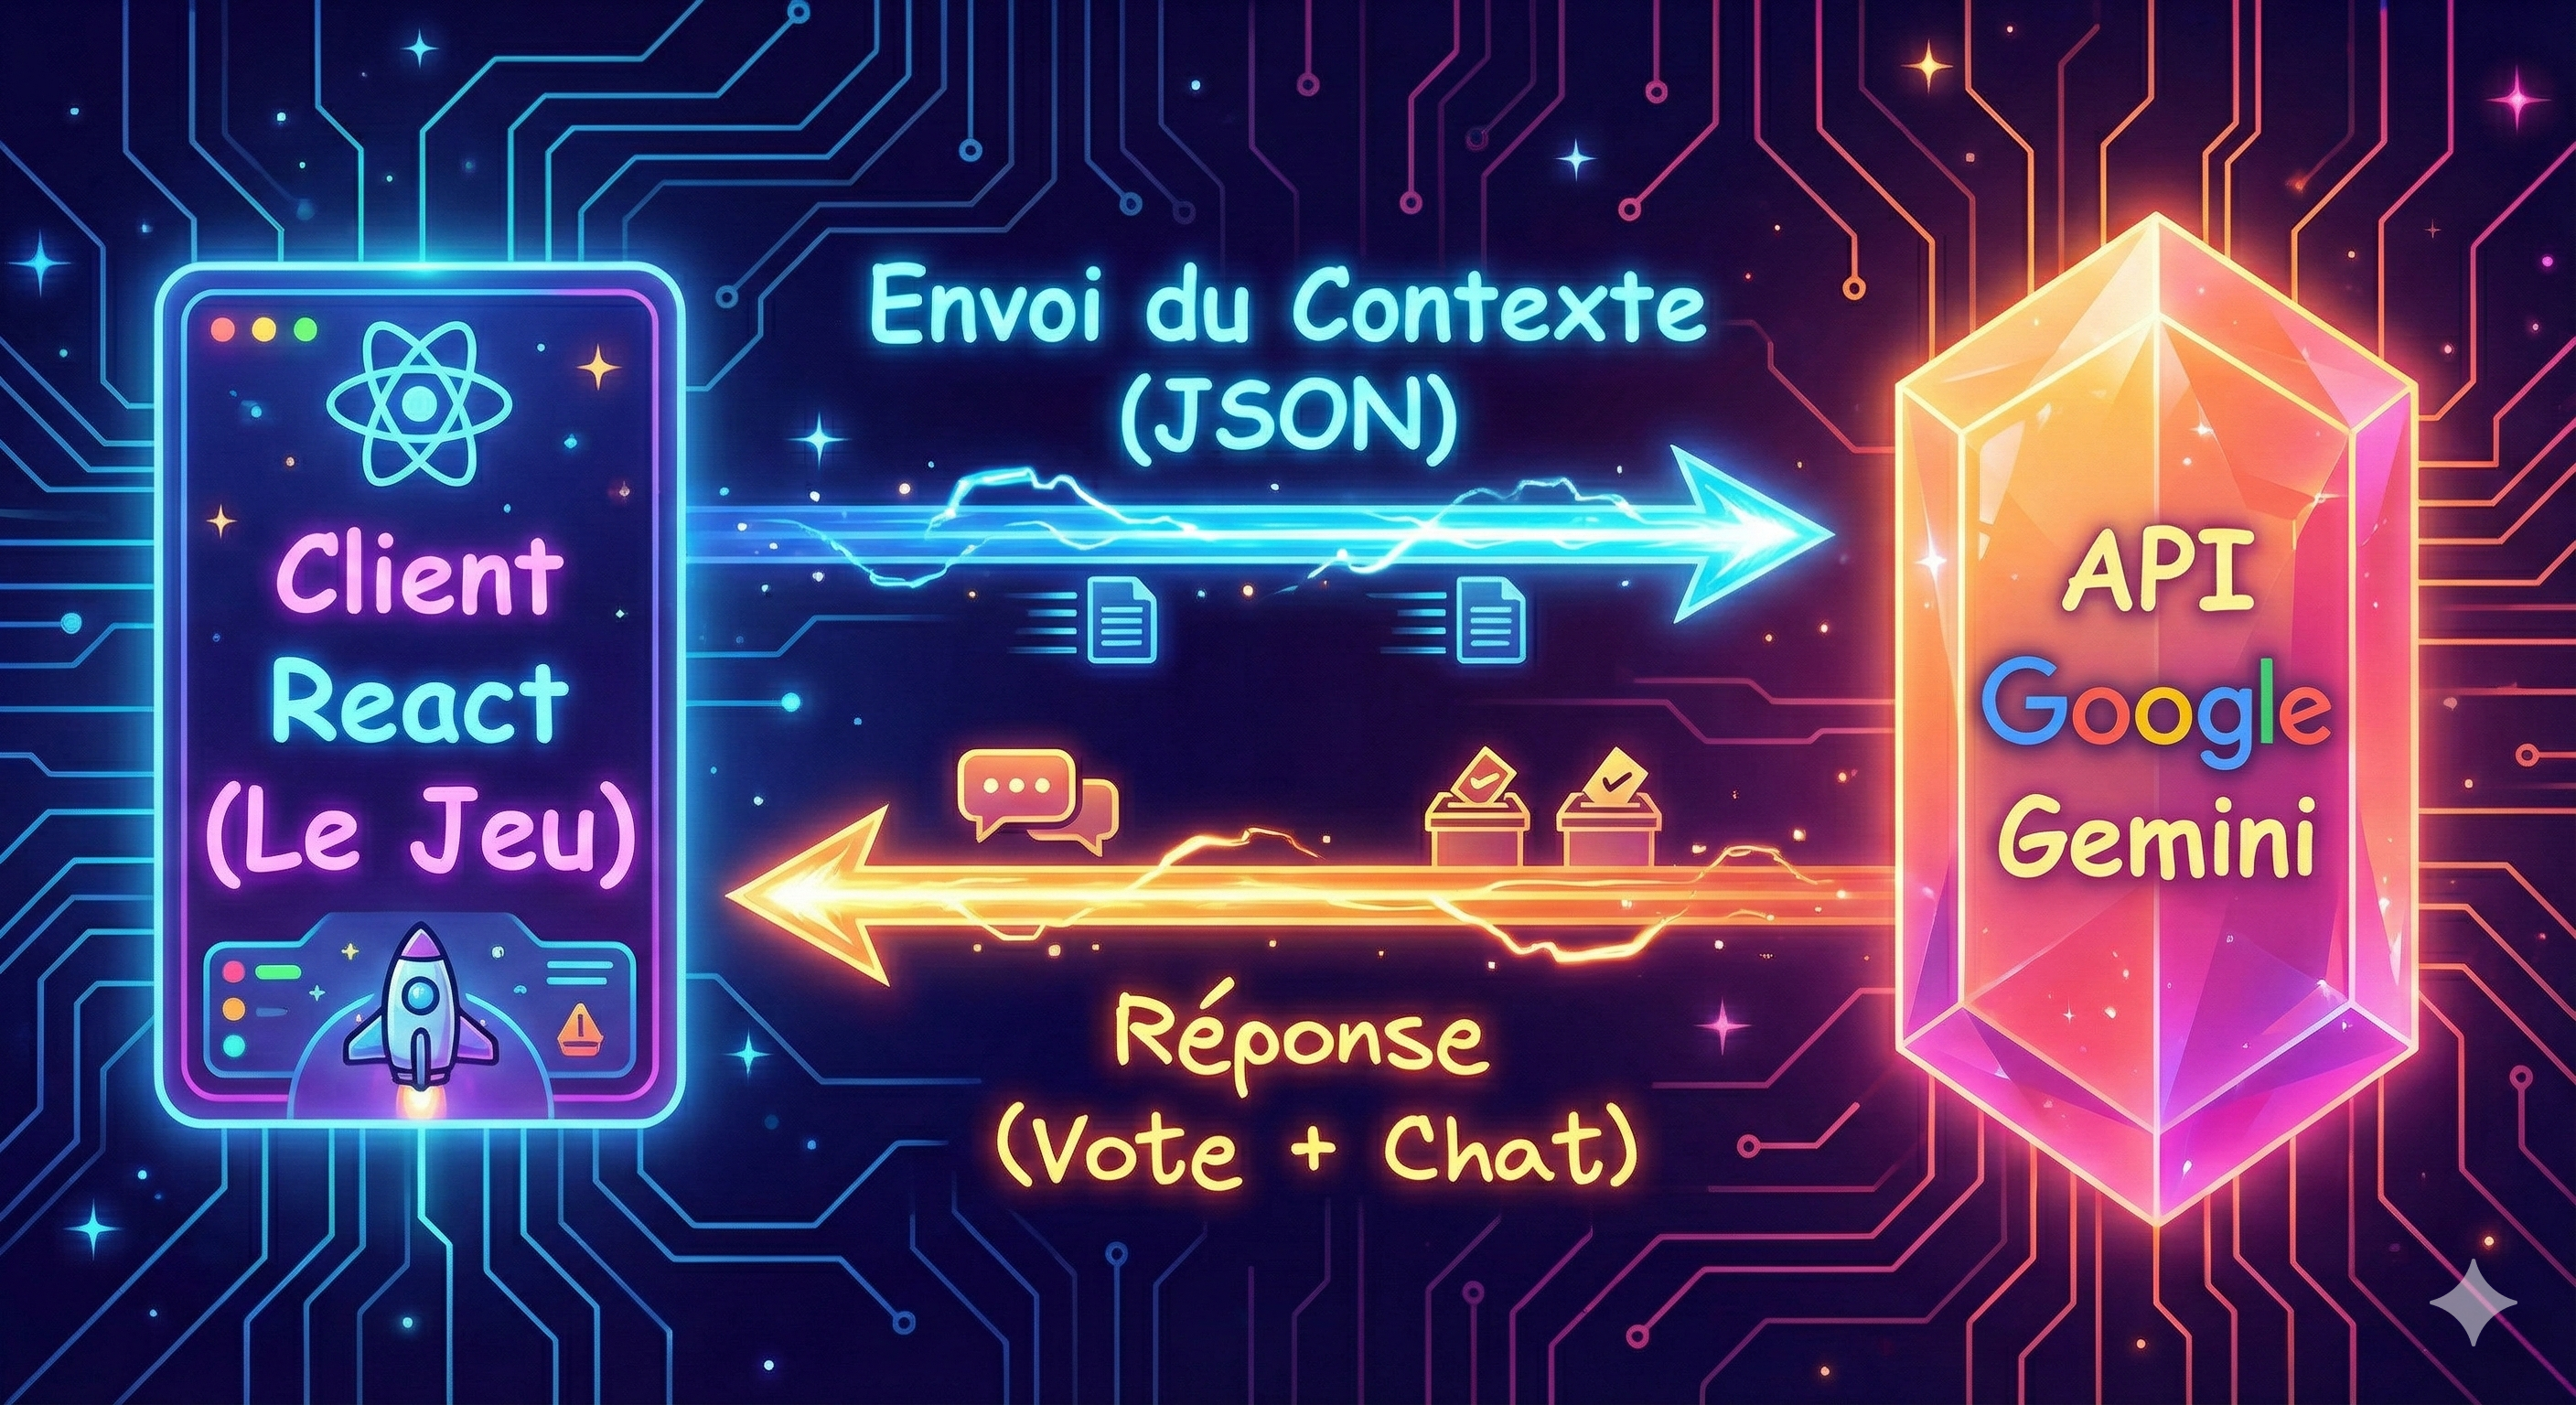
\includegraphics[width=0.8\textwidth]{architecture_ia.png}
    \caption{Flux de données entre le jeu Secret Hitler et l'API Gemini}
\end{figure}




\section{Description du projet et objectifs}

\subsection{Fonctionnement général du jeu}
\includegraphics[width=0.35\textwidth]{liberal.png}
\includegraphics[width=0.35\textwidth]{fascist.png}
\includegraphics[width=0.33\textwidth]{hitler.png}


Le projet consiste à développer une application web reproduisant le jeu de société 
\textit{Secret Hitler}. Le jeu se déroule en plusieurs tours durant lesquels les joueurs 
doivent voter, prendre des décisions collectives et tenter d’identifier les rôles secrets.
L’application gère automatiquement les différentes phases du jeu, les votes, ainsi que 
l’évolution de la partie en respectant les règles officielles.

\subsection{Objectifs pédagogiques et techniques}
Ce projet a pour objectif de mettre en pratique les connaissances acquises en programmation 
web et en théorie des graphes. La figure ci-dessous synthétise les quatre piliers fondamentaux de ce travail, alliant compétences techniques, modélisation mathématique et méthodologie collaborative.

\begin{figure}[H]
    \centering
    % Assurez-vous que le fichier image_0dc403.jpg est bien dans votre dossier
    \includegraphics[width=1\textwidth]{image_0dc403.jpg}
    \label{fig:objectifs_projet}
\end{figure}


\section{Difficultés rencontrées et Solutions Techniques}

Dans le cadre du développement de l'adaptation web de \textit{Secret Hitler}, nous avons rencontré plusieurs défis techniques et conceptuels. Voici le détail de ces obstacles et des solutions apportées.

\vspace{3cm}

% --- 1. GRAPHE ---
\subsection{La Modélisation et la Visualisation du Graphe de Confiance}
\textbf{La Difficulté :} Il fallait représenter graphiquement les relations entre les joueurs (qui soupçonne qui) via des courbes dynamiques. La difficulté résidait dans le calcul mathématique des relations et la gestion de la "visibilité sélective".

\textbf{La Résolution :}
Nous avons défini un graphe orienté et pondéré. Chaque arête possède un poids entre -1.0 (Conflit) et +1.0 (Alliance) (Figure \ref{fig:graph_def}).

\begin{figure}[H]
    \centering
    \includegraphics[width=0.75\textwidth]{image_831da8.png} 
    \caption{Définition technique des arêtes pondérées}
    \label{fig:graph_def}
\end{figure}

De plus, la logique du jeu influence directement ces couleurs (orange, vert) (Figure \ref{fig:logic_color}).

\begin{figure}[H]
    \centering
    \includegraphics[width=0.75\textwidth]{image_831dc6.png}
    \caption{Règles d'évolution du graphe selon les lois votées}
    \label{fig:logic_color}
\end{figure}

% --- 2. IA / BOTS ---
\subsection{L'Intelligence Artificielle des Bots (Prise de Décision)}
\textbf{La Difficulté :} Créer des bots qui ne jouent pas totalement au hasard, mais qui simulent un comportement humain cohérent (méfiance envers les fascistes).

\textbf{La Résolution :}
Création d'une \textbf{Matrice de Confiance} (\texttt{trustMatrix}). Le vote des bots est calculé selon la moyenne des confiances envers le Président et le Chancelier.

\begin{figure}[H]
    \centering
    \includegraphics[width=0.8\textwidth]{image_83a7cc.png}
    \caption{Détail de l'algorithme de vote pondéré}
    \label{fig:ia_algo}
\end{figure}

% --- 3. RYTHME ---
\subsection{Le Rythme du Jeu et la Narration (UX)}
\textbf{La Difficulté :} Initialement, le code exécutait les tours instantanément. L'information défilait trop vite dans les logs pour être comprise par le joueur.

\textbf{La Résolution :}
Développement d'un système de \textbf{"Queue d'Annonces"}. Le jeu se met en pause visuelle pour afficher les événements majeurs.


\begin{figure}[H]
    \centering
    \includegraphics[width=0.85\textwidth]{image_8d870c.png}
    \caption{Overlay d'annonce : Une loi Fasciste est promulguée}
    \label{fig:overlay_loi}
\end{figure}

% --- 4. ALÉATOIRE ---
\subsection{Gestion de l'Aléatoire et Mise en Scène}
\textbf{La Difficulté :} Manque de sensation d'aléatoire lors de l'attribution des rôles (sentiment de répétition).

\textbf{La Résolution :}
Correction de l'algorithme de mélange (\textit{Fisher-Yates}) et création d'une animation "Roulette" pour matérialiser le hasard.

\begin{figure}[H]
    \centering
    \begin{minipage}{0.48\textwidth}
        \centering
        \includegraphics[width=\linewidth]{image_8e09f2.png}
        \caption{Attribution Libéral}
    \end{minipage}\hfill
    \begin{minipage}{0.48\textwidth}
        \centering
        \includegraphics[width=\linewidth]{image_8e09eb.png}
        \caption{Attribution Hitler}
    \end{minipage}
\end{figure}

% --- 5. REACT / SYNCHRONISATION ---
\subsection{La Synchronisation des États et les Boucles Infinies}
\textbf{La Difficulté :} Le jeu fonctionne comme une "machine à états" séquentielle, alors que React cherche à mettre à jour l'affichage instantanément. Nous avons rencontré des problèmes de \textbf{boucles infinies} (re-renders en chaîne) causées par des bots modifiant l'état trop rapidement.

\textbf{La Résolution :}
Nous avons dû imposer un séquençage strict :
\begin{itemize}
    \item Utilisation de délais (\texttt{setTimeout}) pour découpler la logique de jeu du rendu.
    \item Pauses obligatoires pour permettre aux animations (Flash Info) de se terminer.
\end{itemize}

\begin{figure}[H]
    \centering
    \includegraphics[width=0.9\textwidth]{image_8e8252.png}
    \caption{Exemple d'événement asynchrone (Flash Info) géré sans bloquer le rendu}
    \label{fig:flash_info}
\end{figure}

% --- 6. AUDIO ---
\subsection{La Gestion de l'Audio et l'Autoplay}
\textbf{La Difficulté :} Les navigateurs bloquent la lecture automatique (Autoplay Policy). De plus, les changements de page React coupaient la musique.

\textbf{La Résolution :}
Création d'un écran "Start" obligeant l'interaction et mise en place d'un \textbf{Singleton Audio}.

\begin{figure}[H]
    \centering
    \includegraphics[width=1.0\textwidth]{edited-image.png}
    \caption{Écran d'accueil forçant l'interaction utilisateur pour activer l'audio}
    \label{fig:audio_start}
\end{figure}

\begin{figure}[H]
    \centering
    \includegraphics[width=0.95\textwidth]{zoom_texte.png} 
    \caption{Agrandissement du message d'avertissement à l'utilisateur}
    \label{fig:audio_zoom}
\end{figure}

\vspace{5em}

\section{Bilan}
Ce projet a permis de développer une application web inspirée du jeu de société 
\textit{Secret Hitler}, en combinant programmation web, théorie des graphes et 
utilisation de l’intelligence artificielle. La modélisation des interactions entre 
joueurs sous forme de graphes a permis d’appliquer concrètement les notions vues en cours. 
Le travail en groupe et l’assistance par l’IA ont également contribué à la réussite du projet.


\section{Annexes}
\subsection{Exemple d’exécution du projet}
\begin{figure}[h]
    \centering
    \includegraphics[width=0.8\textwidth]{lancement.png}
    \caption{Lancement du jeu}
    \label{fig:execution-jeu}
\end{figure}

\begin{figure}[h]
    \centering
    \includegraphics[width=0.3\textwidth]{liberal.png}
    \includegraphics[width=0.29\textwidth]{fascist.png}
    \includegraphics[width=0.28\textwidth]{hitler.png}
    \caption{Détermination du rôle}
    \label{fig:execution-jeu}
\end{figure}

\begin{figure}[h]
    \centering
    \includegraphics[width=0.7\textwidth]{conseil.png}
    \caption{Les Aides et Analyses}
    \label{fig:execution-jeu}
\end{figure}

\begin{figure}[h]
    \centering
    \includegraphics[width=0.9\textwidth]{deroulement.png}
    \caption{Le déroulement du jeu}
    \label{fig:execution-jeu}
\end{figure}

\begin{figure}[h]
    \centering
    \includegraphics[width=0.7\textwidth]{pioche.png}
    \includegraphics[width=0.7\textwidth]{pioche2.png}
    \caption{La pioche et le décompte (30sec)}
    \label{fig:execution-jeu}
\end{figure}



\large\subsection{Manuel utilisateur}
\subsubsection{Rôles des joueurs}

Chaque joueur reçoit secrètement un rôle au début de la partie :
\begin{itemize}
    \item Les \textbf{Libéraux} ne connaissent l’identité de personne.
    \item Les \textbf{Fascistes} connaissent les autres fascistes.
    \item \textbf{Hitler} ne connaît pas les fascistes (dans les parties à plus de six joueurs).
\end{itemize}

\vspace{3cm}

\subsubsection{Déroulement d’un tour}

À chaque tour :
\begin{itemize}
    \item Un Président est désigné.\vspace{1cm}\\
    \includegraphics[width=0.27\textwidth]{choix.png}
    *
    \item Le Président propose un Chancelier. \vspace{1cm} \\
    \includegraphics[width=0.27\textwidth]{ja.png}
    \item Tous les joueurs votent pour accepter ou refuser le gouvernement. \vspace{1cm}\\
    \includegraphics[width=0.3\textwidth]{loi.png}
    
    \item En cas d’acceptation, des lois sont piochées et une loi est adoptée.
\end{itemize}

\vspace{3cm}

\subsubsection{Conditions de victoire}

La partie se termine lorsqu’une des conditions suivantes est atteinte :

\begin{itemize}
    % --- BLOC LIBÉRAL ---
    \item \textbf{Victoire des Libéraux :} Ils gagnent si 5 lois libérales sont adoptées ou si Hitler est éliminé.
    
    % 1. Image du tableau des lois Libéral
    \begin{figure}[H]
        \centering
        \includegraphics[width=0.6\textwidth]{loi_liberal.png}
        \caption{Tableau des lois Libérales}
    \end{figure}

    \vspace{0.5cm} % Petit espace entre les deux images

    % 2. Image de l'écran de victoire Libéral
    \begin{figure}[H]
        \centering
        \includegraphics[width=0.8\textwidth]{nom_image_liberal.png}
        \caption{Écran de Victoire Libérale}
        \label{fig:victoire_liberale}
    \end{figure}

    % --- BLOC FASCISTE ---
    \item \textbf{Victoire des Fascistes :} Ils gagnent si 6 lois fascistes sont adoptées.

    % 1. Image du tableau des lois Fasciste
    \begin{figure}[H]
        \centering
        \includegraphics[width=0.6\textwidth]{loi_fascist.png}
        \caption{Tableau des lois Fascistes}
    \end{figure}

    \vspace{0.5cm} % Petit espace entre les deux images

    % 2. Image de l'écran de victoire Fasciste
    \begin{figure}[H]
        \centering
        \includegraphics[width=0.8\textwidth]{nom_image_fasciste.png}
        \caption{Écran de Victoire Fasciste}
        \label{fig:victoire_fasciste}
    \end{figure}
\end{itemize}

\section{Conditions Spéciales (Clé API Gemini)}

Bien que le cœur du jeu "Secret Hitler" soit entièrement fonctionnel de manière autonome, le projet intègre une couche optionnelle d'Intelligence Artificielle générative via l'API Google Gemini. L'ajout d'une clé API enrichit l'immersion narrative et l'interaction stratégique.

\vspace{2cm}

\subsection{Génération Narrative : La Chute de la République}

Il existe une condition de victoire alternative et immédiate pour les Fascistes : si Hitler est élu Chancelier après que 3 lois fascistes ont déjà été votées, la partie s'arrête instantanément.

Au lieu d'un simple message de fin, l'IA prend le relais pour rédiger un article de journal unique, annonçant la chute tragique de la République et l'instauration du nouvel ordre. Cela rend chaque conclusion historiquement marquante.

% --- VOS IMAGES ORIGINALES (CONSERVÉES) ---
\begin{figure}[H]
    \centering
    \begin{minipage}{0.48\textwidth}
        \centering
        \includegraphics[width=\linewidth]{image_4d213e.png}
        \caption{Exemple de variation d'article généré par Gemini.}
    \end{minipage}\hfill
    \begin{minipage}{0.48\textwidth}
        \centering
        \includegraphics[width=\linewidth]{image_578b28.png}
        \caption{Article : "Tragédie Nationale" généré par l'IA}
    \end{minipage}
\end{figure}

\vspace{2cm}

\subsection{L'Analyste Stratégique et Narratif (IA)}

Une fonctionnalité d'assistance est accessible en cours de partie via le bouton violet et les événements de jeu. L'IA analyse la situation en temps réel pour offrir deux types d'interventions :

\begin{itemize}
    \item \textbf{Le Conseil Stratégique :} En cliquant sur l'icône, l'IA analyse les logs récents (votes, lois) et suggère une stratégie adaptée au rôle du joueur (ex: se fondre dans la masse pour un fasciste).
    \item \textbf{La Narration Contextuelle :} Lorsqu'une loi passe, l'IA génère un "Flash Info" unique sous forme de propagande radio, renforçant l'immersion.
\end{itemize}

\begin{figure}[H]
    \centering
    \begin{minipage}{0.48\textwidth}
        \centering
        % Remplacez par le nom de votre image de conseil (ex: image_7592c7.jpg)
        \includegraphics[width=\linewidth]{image_7592c7.jpg}
        \caption{Conseil tactique généré par l'IA pour un Fasciste.}
    \end{minipage}\hfill
    \begin{minipage}{0.48\textwidth}
        \centering
        % Remplacez par le nom de votre image de flash info (ex: image_695120.jpg)
        \includegraphics[width=\linewidth]{image_695120.jpg}
        \caption{Flash Info narratif réagissant à une loi votée.}
    \end{minipage}
\end{figure}

\vspace{6cm}

\begin{center}
    % \fboxsep = espace intérieur / \fboxrule = épaisseur du trait
    \setlength{\fboxsep}{15pt}
    \setlength{\fboxrule}{2pt}
    
    % Boite : Cadre Rouge (red), Fond Gris clair (black!5)
    \fcolorbox{red}{black!5}{
        \begin{minipage}{0.7\textwidth} % La boite prend 70% de la largeur de la page
            \centering
            \Large \itshape \bfseries \textcolor{red!80!black}{
                P.S. : Je vous jure que je suis Libéral. \\
                \small(Mais c'est exactement ce que dirait Hitler...)
            }
        \end{minipage}
    }
\end{center}

\vspace{1cm}

\end{document}